\chapter{Methodology}\label{method}
\label{Methodology}
In previous chapters we introduced our research problem, listed and explained the solution options with the theoretical background. In this chapter we shall try to explain our practical approach for carrying out the research along with the software development required to support the experimentation and data analysis for our research. On a practical level following were some major tasks that were required to fulfil scope of our research.
\begin{itemize}
\item Understanding energy efficiency, smart grids and available data.
\item Requirement engineering and use case preparation.
\item Understanding Data Analytics ecosystem, evaluating the big data tools and solutions.
\item Exploratory data analysis and selection of algorithms and data analysis tools with respect to use cases. 
\item Developing an end to end big data analytics platform.
\item Data collection, storage and preprocessing.
\item Use case specific data analysis and evaluation of results.
\item Visualization of results 
\item Documentation of the research, process, software development and results.
\end{itemize}
Some of these tasks were required to be performed in a sequential way e.g. requirement engineering and evaluation of big data tools were required before developing the big data analytics platform or selecting the algorithms. Similarly we need to have results before visualizations could be created. On the other hand some of the tasks could have been executed in parallel. For example the documentation was an ongoing process along with all other tasks. Similarly literature review for understanding each component of our research was also an ongoing process through the time line for this thesis. The regardless of sequential and parallel tasks we need to iterate for continuous improvement.

To tackle these challenges we needed a methodology that can support sequential and parallel task execution with support for iterations to improve. Like most of scientific researches, fail fast and small to succeed was the key for us. In the list of tasks mentioned above. Most of them requires conceptualization and tested quickly using rapid prototyping. Taking it as a software development task initially, we had some candidate models such as water fall model,agile development model, spiral model and incremental model etc. Here we shall briefly discuss the advantages and disadvantages in context to our research project. 
\begin{itemize}
\item \textbf{Waterfall model} offered the simplest approach of requirement engineering, design, implement, test and operate our research. How ever it is inherently sequential and had weak support for iterations.
\item \textbf{Agile development model} Agile methodology\cite{martin2003agile} is rapid, iterative and supports quick prototyping but it requires additional communication and management overhead like scrum meetings. Managing it along with stakeholders like VTT and CIVIS projects was very hard.
\item \textbf{Spiral Model} is a risk driven process model.It supports prototyping, provides good way of avoiding major failure risks, it is iterative. However it needs a lot of resources during planning phase specially when the spiral keeps growing in size. It is usually very successful for large projects but it has over heads for small projects like our thesis research. We shall be discussing more about using parts of the spiral model later in this chapter.
\item \textbf{Incremental model} relies on small incremental steps with each step consist of independent design, implement and test phase. In the begining, Incremental model was the best fit among other candidate models for our thesis research.We were able to prototype small functional units of the big data analytics platform very quickly while independently working on the use cases. However during platform development and data analysis part. It has started creating integration over heads. For example integrating two different data processing tools together for a single use case becomes difficult  when they were configured in two different incremental steps.  
\end{itemize}
Learning from the problems that we face from  incremental model we altered our approach to adapted version of another very flexible software research and development methodology known as ``Kumiega-Van Vliet Trading System Development Methodology''\cite{kumiega2008software}.

\section{Kumiega-Van Vliet Model}\label{kvvm}   
      
Kumiega-Van Vliet Trading System Development Methodology \((K|V)\) was developed in 2008 for software development required specifically for trading systems. It is the combination of three general purpose software and new product development models i.e. waterfall model, spiral model and stage gate model. We have already explained the waterfall and spiral models. Stage gate model consists of stages e.g. scoping, development, implementation, testing etc. Each stage or combination of stages can be controlled with an approval gate. Process can not move from a stage to other stage if the gate in between them is not approved.This model provides a good control over the development model to ensure quality. However it may cause delays because of the organizational hierarchies dictating the gates.

 \((K|V)\) model tries to overcome the short comings of these three models by combining them to a single paradigm for trading system development\cite{kumiega2008software}. In spiral model in start smaller time is allocated to four basic steps i.e. research planning implementation and test. These four steps can be performed again and again in cycles. To avoid spiral to grow two much after each cycle a stage gate controls if process can be passed to next stage or it needs to be sent back to perform another cycle in same stage. Just like waterfall there can be number of stages. But for continuous improvements process there is an iteration channel available unlike traditional waterfall model.
 \section{Adaptation of Kumiega- Van Vliet Model}\label{adaptation}
 \((K|V)\) model is designed for software research  and development in domain of financial services. With the built in stage gate controls it requires some scale of hierarchical organizational structure to support the model. For our highly academic research case we have made certain adjustments. The most notable adaptation was to use deliverables and team reviews of respective deliverables as the main control for moving from one stage to other instead of stage gate approvals in \((K|V)\) model. The waterfall model alike stages helped in keeping our focus on the solution for our problem statement. The spiral model cycles enabled us to iterate within a stage and improve the deliverables quality. Typically the decision of additional cycles was based on the feedback during the team review sessions. The inter stage iteration channels helped us in improving our overall quality. The lessons learnt or the new directions identified during one iteration was include in the scope of research for next iteration. It also allowed us to include supplementary topics in our scope without losing focus on mandatory issues.
 
 In our approach, we have divided complete scope of research in four basic stages. Within each stage we had four steps. These intra stage steps were different for each stage. These steps were corresponding to the main tasks that we discussed in start of this chapter. A typical intra stage cycle ended with a set of deliverables. The deliverables were reviewed in a team review session. If required the other stockholders like VTT were also involved in some of the review meetings. We shall be discussing it in details when we describe our stage wise proceedings. At end of each review session a decision was made to either move to next stage or try to improve via additional cycle. Using all four intra stage steps for additional cycles was not a must. This was another minor adaptation to the \((K|V)\) model. Similarly iterations were mostly initiated after stage three. There were three major iterations. During the iterations change of deliverables were not mandatory. However in practice it was observed that iteration had caused some major or minor changes in stage deliverables as well. Small informal team structure reduced management and communication efforts. This also helped in rapid processing during iterations. Figure~\ref{fig:kv} illustrates our approach with the adapted version of \((K|V)\) model. Stage by stage description of our research methodology is explained in next section.   
 \begin{figure}[!h]
   \begin{center}
     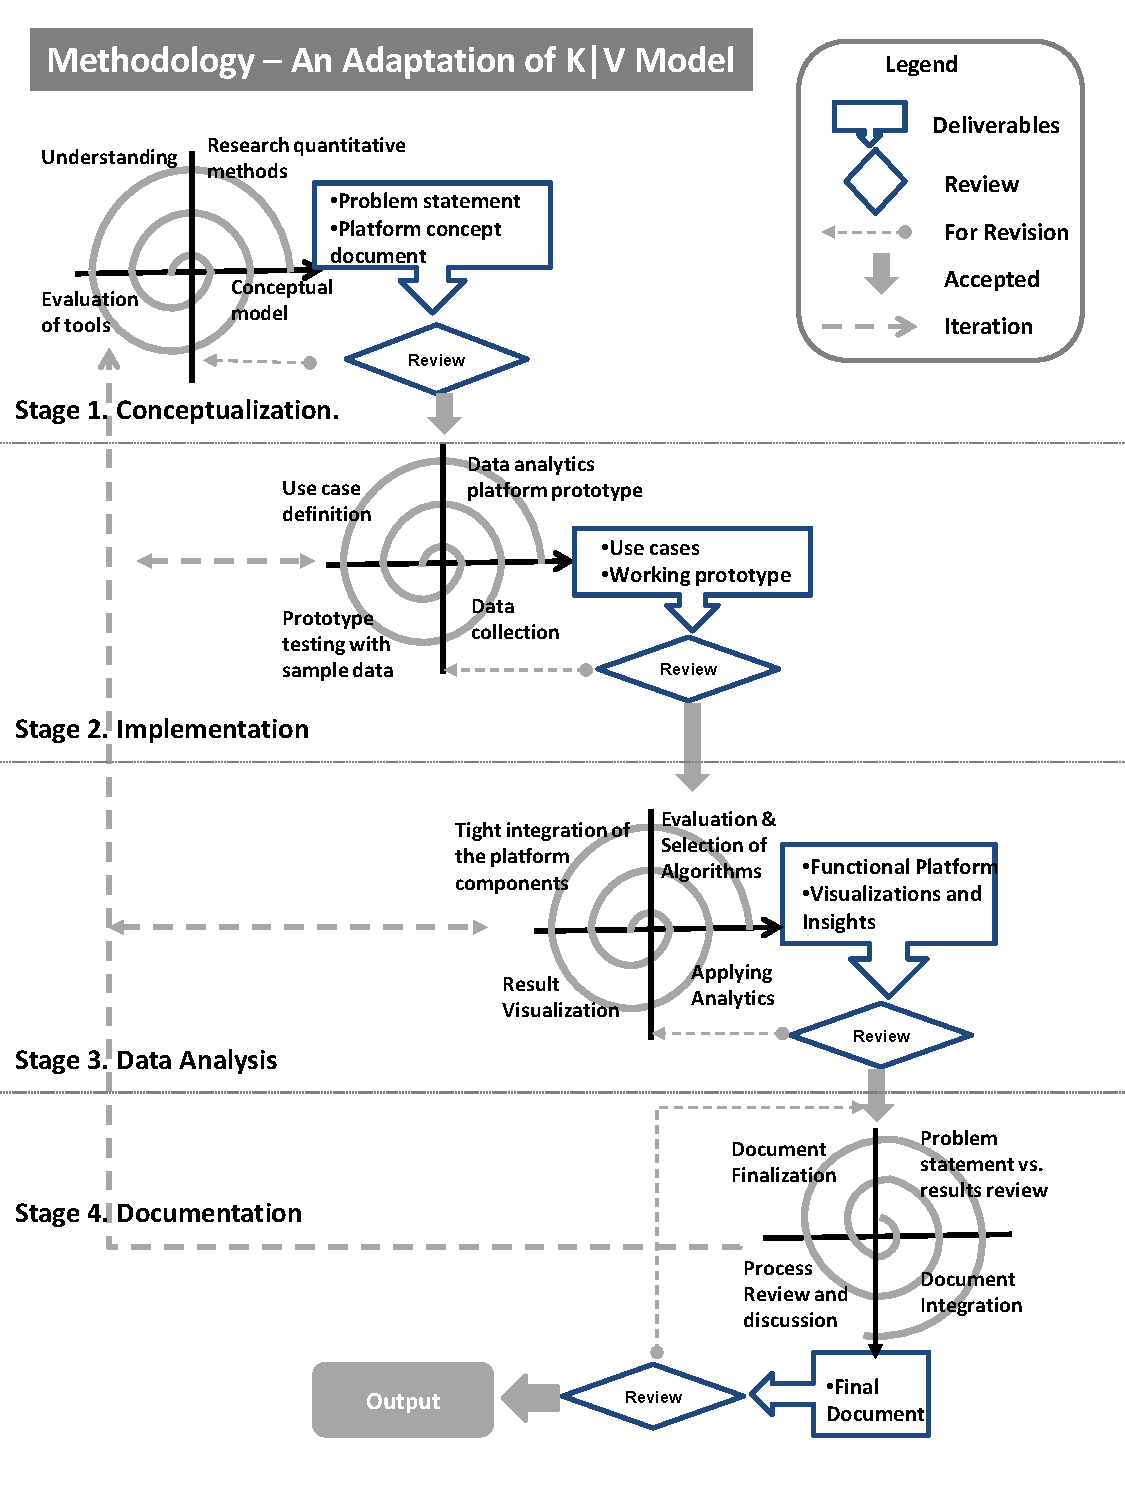
\includegraphics[width=\textwidth]{images/kv_method.pdf}
     \caption{Methodology, An Adaptation of \(K|V\) Model}
     \label{fig:kv}
   \end{center}
 \end{figure} 
\section{Stages, steps and cycles}\label{stages} 
We have already mentioned that there were four stages with each having four respective steps. Each stage was controlled via deliverables review sessions in a stage gate manner. While inside a stage, steps were executed in spiral cycles. First cycle of the spiral had to pass through the four steps. The additional cycles are initiated if the further improvements are decided for deliverables in review session. All Four steps were not mandatory for additional cycles. In this section we shall be listing and describing the stages along with respective steps. We shall be highlighting some major cycles and deliverables. However the iterations will be discussed in next section. Figure ~\ref{fig:kv} will be our main reference through out this section. In this section we shall mention some functional components of our project e.g. logical architecture, data processing tools and algorithms etc. Details for these functional components will be given in later part of this document.
\subsection{Stage 1. Conceptualization } \label{concept}
In start our research problem was mainly concerned about processing large volumes of data coming from smart metering devices and understand the consumption patterns. So the primary focus of the conceptualization stage was to describe our problem in detail, understand important factors related to it, find and evaluate methods and tools to solve the problem. The stage had following four steps.
\subsubsection{Step 1. Understanding} 
From the start, our research had two focus areas i.e. energy consumption and big data . The main purpose of this step was to understand important concepts related to these topics. Follwoing are some main activities performed during this step.
\begin{itemize}
\item Intensive literature review.
\item Participation in CIVIS project Helsinki- Use case workshop 26-27 January 2014. It gave good insights about ecological and social factors effecting energy production, distribution and consumption.
\item Participation in VTT Green Campus Initiative Introduction session.
\item Discussions and informal interviews with VTT's project lead for Green Campus Initiative.
\item Aalto University courses.
	\begin{enumerate}
	    \item Scalable Cloud Computing, as a good introduction to parallel batch processing and its uses for big data processing.
	    \item Information Visualization, as an introduction to effective communication through data visualization.
	  \end{enumerate}      
\end{itemize}

Literature review had been a constant step through out this stage, cycles, and iterations.
\subsubsection{Step 2. Research quantitative methods} \label{qm}
This step involved finding and evaluating the various quantitative methods used for measuring energy consumption and benchmarking energy efficiency. Data aggregation methods like daily, monthly consumption, and average consumption etc were evaluated. Identification and theoretical evaluation of advance analytical methods was also performed during this step.
\subsubsection{Step 3. Conceptual Model}\label{cmodel}
This step was dedicated for finding available open source solutions to make a conceptual model for an end to end big data analytics. This step was mandatory for the big data platform concept paper deliverable. This step was also repeated during various iterations, whenever change was required in data platform.
\subsubsection{Step 4. Evaluation of Tools}
This step was in pair with \ref{cmodel}. All the tools listed in conceptual model were tested during this step. A checklist of evaluated and selected tools was maintained. This list is available as annex???

\subsubsection{Delivearbles of stage 1}
There were two deliverables of this stage
\begin{enumerate}
\item Problem Statement. first two steps of this stage were the main contributors for this deliverable.
\item Platform concept document. A document as result of step 3 and 4 of this stage. 
\end{enumerate}

\subsubsection{Stage 1 cycles}
In this stage we observed two cycles i.e. cycle for producing the required deliverables and one additional cycle for modification of platform concept document. The main modification in additional cycle was the replacement of application frame work with an architecture diagram to clarify.
\subsection{Stage 2. Implementation}\label{implement}
This stage mainly includes requirement engineering and intensive software development to prototype and test the big data platform described in concept paper as a deliverable from stage 1. This stage had following four steps.
\subsubsection{Use case definition} 
In this step, Based on the knowledge gained from stage 1. we decomposed our problem statement into lower level requirements that can be practically implemented using big data platform concept. Use cases went through several iterations. Details of iterations will be discussed later in this chapter. However here we shall list the final list of use cases.
\begin{enumerate}
\item Understanding the seasonal energy usage patterns and its sensitivity with outside temperature.
\item Understanding characteristics of building using daily energy consumption pattern.
\item Calculate the base load of the building to identify non user consumption of buildings
\item Classify building on basis of energy efficiency and analyse seasonal shifts in this classification.
\item Predict daily energy consumption of various house hold devices on basis of previous consumption pattern.
\end{enumerate}
\subsubsection{Data Analytics Platform Prototype}
This step involved the practical implementation of platform concept. It covered installation, configuration, customization and integration of selected components as a proof of concept for an end to end big data platform that can collect, store, process, analyse and visualize data. Details of the components and implementation will be discussed in next chapter.
\subsubsection{Data Collection}
As mentioned before, real life energy consumption data was provided by VTT. This data was collected by VTT from the smart metering devices installed on test sites. We had prepared our prototype platform to collect this from VTT data repositories continuously in real time. However due to some policy constraints we were not allowed to integrate our platform with VTT's data repositories. The data was provided to us initially via file transfer from a FTP\footnote{The File Transfer Protocol (FTP) is a standard network protocol used to transfer computer files from one host to another host over a TCP-based network, such as the Internet.} server. In later a web sevice was opened for us to collect the data. the details of the data will be provided later in the document however two types of data were collected during different iterations.
\begin{enumerate}
\item Hourly consumption of electricity, electricity used for heating, water, and reactive power in set of buildings as part of VTT's green campus initiative.
\item Device level electricity consumption data of home appliances used in two apartments of Aalto Univerity campus residential housing blocks as test cases for VTT's green campus initiative.
Real time data was also collected using the same platform to support some CIVIS projects objectives. However the real time data was not included in scope of analysis presented in this document.  
\end{enumerate}
\subsubsection{Prototype testing with sample data}\label{prototype}
This step was only used during first cycle of this stage and first iteration of whole process. The purpose of this stage was to test the full flow from data collection to data visualization using the developed prototype. The sample data was the randomly selected records from hourly consumption data set. Although in this step we started with smaller sample and then kept on increasing it. The complete data set was also tested. In testing following functionalities were tested.
\begin{enumerate}
\item Data collection.
\item Raw data storage
\item Data cleaning to produce tidy data set.
\item Data pre-processing. Reducing the large data volume without losing insights. 
\item Storing pre-processed data into databases.
\item Testing of advance analytics tools integrated within our prototype.
\item Data visualization.  
\end{enumerate}
\subsubsection{Stage 2 deliverables}
Following were two deliverables of implementation stage.
\begin{enumerate}
\item Use case definition
\item Working Prototype of big data platform concept.
\end{enumerate}
\subsubsection{Stage 2 cycles}
Stage went through two additional cycles on top of the first mandatory cycle. Within two additional cycles all the steps were performed except data collection that was collected once during the this stage for first cycle. However data collection was repeated within iteration that will be discussed in later in this chapter.
The major revisions inside cycles includes alteration in use cases e.g. effect of external temperature on seasonal energy pattern was identified during one of the review sessions. Within prototype and protype testing the alterations were required the adapt for changes in use cases

\subsection{Stage 3 Data Analysis}
In this stage we used the data platform to analyse the collected data and produce the insights based on use cases. We applied the basic and advanced analytics techniques introduced in \ref{daily},\ref{seasonal},\ref{classify},\ref{predict} sections. This stage has following four steps.
\subsubsection{Tight integration of the platform components}
In section \ref{prototype} we tested all the units of the platform by manually enforcing the process i.e. taking out the  output of one module manually as in input to the other module on requirement basis. In this step we tried to automate the process by coupling the modules together in form of a single process per use case. 
\subsubsection{Evaluation and selection of algorithms}\label{eval}
In this step we tried to find and compare various options of advance analytics algorithms available for supporting our uses cases. It involved quantitative methods considered in section \ref{qm}. However the focus was more on the advance analytics. The techniques explained in \ref{daily},\ref{seasonal},\ref{classify},\ref{predict} sections were selected during this step. The selection criteria for each algorithm will be discussed in chapter \ref{chapter:Analysis}. For evaluating the algorithms we were using samples from collected data as our training data. 
\subsubsection{Applying Analytics}
In this step we applied the selected algorithm on the complete data sets. The insights generated from this steps are main results for our study. During the cycles of this stage, results from this step also affected the evaluation of algorithms in previous step, section \ref{eval}. Details related to this step will also explained in chapter \ref{chapter:Analysis}.    
\subsubsection{Result Visualization}
For the sake of ease to understand, the extracted insights in te previous step were visualized in form of data graphs. Different tools for visualizations were used in this steps. Visualization tools will be discussed in chapter {chapter:platform}. For data visualization we tried to implement the graphical practices discussed by Edward Tufte in his book ``The visual display of quantitative information''\cite{tufte1983visual}
\subsubsection{Stage 3 deliverables}
There were two deliverables of this stage.
\begin{enumerate}
\item Functional Platform. At the end of this stage, we had a fully functional platform capable of implementing the end to end data analytics.
\item Results and visualization of the results. Providing required insight for the use cases. 
\end{enumerate}
\subsubsection{Stage 3 Cycles}
There were several cycles in this stage. However as deviation from our adaptation of \((K|V)\) model, we just had one review session for this stage per iteration. Combination of different algorithms, their evaluation and then generating visualizations had to be repeated and tested many times. So reviewing in the intermediate cycles was very inefficient. This stage took longer time because of many cycles and the wider spiral required to produce good quality results.
\subsection{Stage 4 Documentation}
Documentation was an on going process throughout the stages and iterations. All of the stages had at least one deliverable in form of some document e.g. stage 1 has big data platform concept paper, stage 2 had use cases document, in stage 3 we had data analysis and insights report. The purpose of the last stage was to consolidate all the information in different documents together in shape of one single thesis report. Following were four steps for this stage. 
\subsubsection{Problem statement vs. results review}\label{ps}
This step was the check for consistency of our results with the research problem that we had in the beginning. We earlier mentioned that documentation stage was not always part of the iterations. However this stage was used during all the iterations to keep track of the main focal points, the complimentary and supplementary parts of our research.    
\subsubsection{Document Integration}
This step was concerned with the main task of this stage i.e. to consolidate the information together in form of one consistent story. During this stage we tried to link the inter stage documentation together along with theoretical background and explanation of the process and functional components of the project.
\subsubsection{Process Review and discussion}
The purpose of this step was to provide a retrospective view of the whole process. Highlight the main findings and discuss what could have been done better or more to improve the process and produce further results. This step also indicate some future directions for the relevant research areas. The considerations of this stage will be discussed further in chapter \ref{chapter:discussion}.
\subsubsection{Document Finalization}
This step controlled the final thesis report publishing aspects like formatting, sequencing of topics, proof reading and version control etc.  
\subsubsection{Stage 4 deliverables}
The final thesis report document was the mandatory deliverable  as the main output of the process and our research project. There were some supplementary deliverables like source codes, code books and procedures etc. that we intended to open source as part of our research.   
\subsubsection{Stage 4 Cycles}
to be written in end
\section{Iterations} \label{iteration}
Iterative processes and work models do not require full specification right from beginning. Instead the implementation can start with small part of specification. Then in a step wise approach the next scope is defined with consideration of lesson learnt and new directions found from previous iterations. This inherent characteristic of iterative processes had a vital role in our research. We started with smaller scope i.e. two simple uses case. In earlier iteration we were able to focus on big data technologies and energy efficiency concepts more than the complex advance analytics topics. Findings and practical implementation in early phase enabled us to expand our scope later. We added more use cases with more focus on data analysis and application of big data for energy efficiency. Iterations also helped us in improving the quality of research. 

In our approach, we went through 3 main iteration cycles. As mentioned in section \ref{stages} each iteration did not involve the complete four stages and their respective steps. First three stages were the main contributors in the iteration with step \ref{ps} of stage 4 as main source for reviewing our proceedings against our targets. Table \ref{tab:iteration_table} list the main activities in each iteration against respective stages and steps.    

%\usepackage{lscape}
%\begin{landscape}
\begin{table}\tiny %[!t]
%\begin{sideways}
\begin{tabular}{|m{2.2cm}|>{\raggedright}m{1.7cm}|>{\raggedright}m{3.4cm}|>{\raggedright}m{3.4cm}|m{3.4cm}|}
\hline
	\textbf{Stages} & \textbf{Steps} & \textbf{Iteration 1} & \textbf{Iteration 2} & \textbf{Iteration 3} \\ \hline
	\multirow{4}{*}{\textbf{Conceptualization}} & Understanding  & Main Topics: Energy Efficiency, Eco-Efficiency, Demand Response, daily consumption, monthly consumption, smart grids, smart metering, NIALM, Big Data 3Vs, Parallel Batch Processing, MapReduce etc & Main Topics: Classification, clustering, K-means, Big Data Veracity and Valuation, Big Data Streaming, Lambda Architecture, Massively Parallel Processing etc. & Main Topics: Forecasting, Regression, Auto-regression, Moving Averages, ARIMA etc. \\ \cline{2-5}
	 & Research quantitative methods
 & Sampling, Aggregation,  Averages, Summation, standard deviation, distributions etc & Clustering,Centroid-based clustering; K-means, C-means, Distribution-based clustering; Cumulative distribution function,  Density-based clustering; DBSCAN.  & Time Series Analysis, Covariance, correlation, Regression, Auto-regression, Moving Averages, ARIMA, Random Forest etc. \\  \cline{2-5}
	 & Conceptual Model & Model for parallel batch processing & Massively Parallel processing added for faster processing & Additional Machine learning modules (Forecasting) \\  \cline{2-5}
	 & Evaluation of Tools & Apache; Hadoop, HDFS, Flume, Sqoop, oozie, Hive, Pig in Cloudera distribution.
R, mahout, Tableau, D3.JS  & Cloudera Impala, Spark, Hbase, MongoDB. & Weka, Cloudera Oryx,  R (Forecast package) \\ \hline
\multirow{4}{*}{\textbf{Implementation}} & Use case definition
 & List of use cases:
(1) Understanding the seasonal energy usage patterns and its sensitivity with outside temperature.
(2) Understanding characteristics of building using daily energy consumption pattern. & List of use cases:
(3) Calculate the base load of the building to identify non user consumption of buildings
(4) Classify building on basis of energy efficiency and analyse seasonal shifts in this classification. & (5) Predict daily energy consumption of various house hold devices on basis of previous consumption pattern. \\ \cline{2-5}
	 & Data analytics platform prototype
 & Parallel batch processing with capability to collect data from data from data servers and public social media streaming API s. Machine learning modules integration . Visualization using Tableau Public. & Integration of on-line query engine with Cloudera Impala. This enabled near to real life big data processing. & Use of additional data mining and machine learning tools like Weka.  \\ \cline{2-5}
	 & Data collection
 & Hourly electricity and  electricity for heating consumption data from VTT's smart metering devices on pilot sites for Green Campus Initiative. & Device level electricity consumption data from VTT's NIALM devices installed in two selected residential apartments. & One month twitter data collection for Green Hackathon using collection of energy related keywords.  \\ \cline{2-5}
	 & Prototype testing with sample data
 & Testing with samples from hourly consumption data. Testing with complete hourly consumption data. & Testing with NIALM device data. & Testing the prediction model using NIALM device data an additional data mining and machine learning tools. Performance comparison between non parallel executing, parallel batch processing and Masively parallel processing tools. \\ \hline
	\multirow{4}{*}{\textbf{Data Analysis}}	 & Tight integration of the platform components
 & End to End workflow implementation i.e. from data collection, storage, preprocessing and analysis to visualization of results. Limited to batch processing only & Integration of Impala.  &  \\ \cline{2-5}
	 & Evaluation \& Selection of Algorithms
 & Selected quantative methods: Basic aggregations e.g. averages , summations and groupings. & Selected quantative method: K-means clustering  & Selected quantative methods:  ARIMA, linear regression and Random Forest forecasting techniques. \\ \cline{2-5}
	 & Applying Analytics
 & Applying basic aggregations according to use case 1 and 2. & 1) Basic Aggregation for use case 3
2) K-means clustering for use case 4 & ARIMA and Random Forest algorithms for use case 5. \\ \cline{2-5}
	 & Result Visualization
 & Using Tableau Public & Using Tableau Public  & Using R plots and Weka \\ \hline
\multirow{4}{*}{\textbf{Documentation}}	 & Problem statement vs. results review
 & Results for use case 1 and 2 reviewed. & Results for use case 3 and 4 reviewed. & Results for use case 5 reviewed. \\ \cline{2-5}
	 & Document Integration
 & Step not used  & Step not used  & Integration of  platform concept paper, data analysis report and use documentation.  \\ \cline{2-5}
	 & Process Review and discussion
 & Step not used  & Step not used  & Theoratical background explainations and linkages to research. Future directions for related work. \\ \cline{2-5}
	 & Document Finalization
 & Step not used  & Step not used  & Document formating. \\ \hline
\end{tabular}
%\end{sideways}
\caption{Details of the iterations}
\label{tab:iteration_table}
\end{table}
%\end{landscape} 